\documentclass[../main.tex]{subfiles}

\graphicspath{{../images/}}

\usepackage[noend]{algpseudocode} % for pseudocode
\usepackage[plain]{algorithm} % float environment for algorithms
% preferred pseudocode style
\algrenewcommand{\algorithmicprocedure}{}
\algrenewcommand{\algorithmicthen}{}

% ``do { ... } while (cond)''
\algdef{SE}[DOWHILE]{Do}{doWhile}{\algorithmicdo}[1]{\algorithmicwhile\ #1}%

% ``for (x in y ... z)''
\newcommand{\ForRange}[3]{\For{#1 \textbf{in} #2 \ \ldots \ #3}}

\begin{document}
\pagestyle{fancy}
\chead{Module 4}
\rhead{Junseo Shin}
\lhead{CSE 4059}


\renewcommand{\thefigure}{\arabic{figure}}
\section*{Tiled Matrix Multiplication}

\subsection*{Questions}

\begin{enumerate}
    \item How many floating operations are being performed in your matrix multiply
    kernel? Explain.
    
    Outside the for loop we have one initialization and one assignment, and inside the for loop
    loop we have $(2 * \texttt{TILE\_WIDTH} + 2) * \texttt{numAColumns / TILE\_WIDTH}$ flops, so
    we end up performing $2 * \texttt{numARows} * \texttt{numBColumns} * \texttt{numAColumns}$
    FLOPs. 

    \item How many global memory reads are being performed by your kernel?
    Explain.

    The two if-else statements at the beginning of the for loop read the global memory
    twice, so one thread performs $2 * \texttt{ceil(numAColumns / TILE\_WIDTH)}$ global memory
    reads. Thus, the kernel performs
    $2 * \texttt{numARows} * \texttt{numAColumns} * \texttt{numBColumns}$ global memory reads.

    
    \item How many global memory writes are being performed by your kernel?
    Explain.

    We have one write at the end of the kernel function, so the kernel performs
    $\texttt{numARows} * \texttt{numBColumns}$ global memory writes.
    
    \item Describe what further optimizations can be implemented to your kernel to
    achieve a performance speedup.

    We can optimize the block size to be a multiple of the warp size (32) and use
    a larger \texttt{TILE\_WIDTH} to reduce the number of global memory reads and writes.
    
    \item Compare the implementation difficulty of this kernel compared to the
    previous MP. What difficulties did you have with this implementation?

    I had trouble keeping track of which matrix width to use for setting up the edge cases
    for the matrix multiplication. In addition, the number of threads per block had to match the
    tile width!

    \item Suppose you have matrices with dimensions bigger than the max thread
    dimensions. Sketch an algorithm that would perform matrix multiplication
    algorithm that would perform the multiplication in this case.

    Using grid-stride loops (\href{https://developer.nvidia.com/blog/cuda-pro-tip-write-flexible-kernels-grid-stride-loops/}{link}),

    \begin{algorithm}
        \caption{Grid-stride loop for tiled matrix multiplication}
        \begin{algorithmic}[1]
            \Procedure{matrixMultGridStride}{}  \Comment{Global kernel function}
                \State $\text{rowStart} = \text{blockIdx.y} \times \text{TILE\_WIDTH}
                    + \text{threadIdx.y}$  
                \Comment{with same shared memory setup}
                \State $\text{colStart} = \text{blockIdx.x} \times \text{TILE\_WIDTH}
                    + \text{threadIdx.x}$ 

                % strides
                \State
                \State $\text{rowStride} = \text{gridDim.y} \times \text{TILE\_WIDTH}$
                \Comment{set up strides}
                \State $\text{colStride} = \text{gridDim.x} \times \text{TILE\_WIDTH}$
                
                % add horizontal space for readability
                \State
                \For{(row $=$ rowStart; numCRows; ++rowStride)} \Comment{Grid-stride loop}
                    \For{(col $=$ colStart; numCColumns; ++colStride)}
                        \State $\text{Cval} = 0$
                        \State $\dots$ \Comment{Same tiling algorithm as before}
                    \EndFor
                \EndFor
                % \For{\texttt{row} \textbf{in} \texttt{0} \ \ldots \ \texttt{numARows} \ \textbf{step} \ \texttt{row\_stride}}
                %     \For{\texttt{col} \textbf{in} \texttt{0} \ \ldots \ \texttt{numBColumns} \ \textbf{step} \ \texttt{col\_stride}}
                %         \State \texttt{matrixMultKernel}(\texttt{A}, \texttt{B}, \texttt{C}, \texttt{numARows}, \texttt{numAColumns}, \texttt{numBColumns})
                %     \EndFor
            \EndProcedure
        \end{algorithmic}
    \end{algorithm}

\end{enumerate}

\newpage

\subsection*{OUTPUT}
\begin{figure}
    [ht]
    \centering
    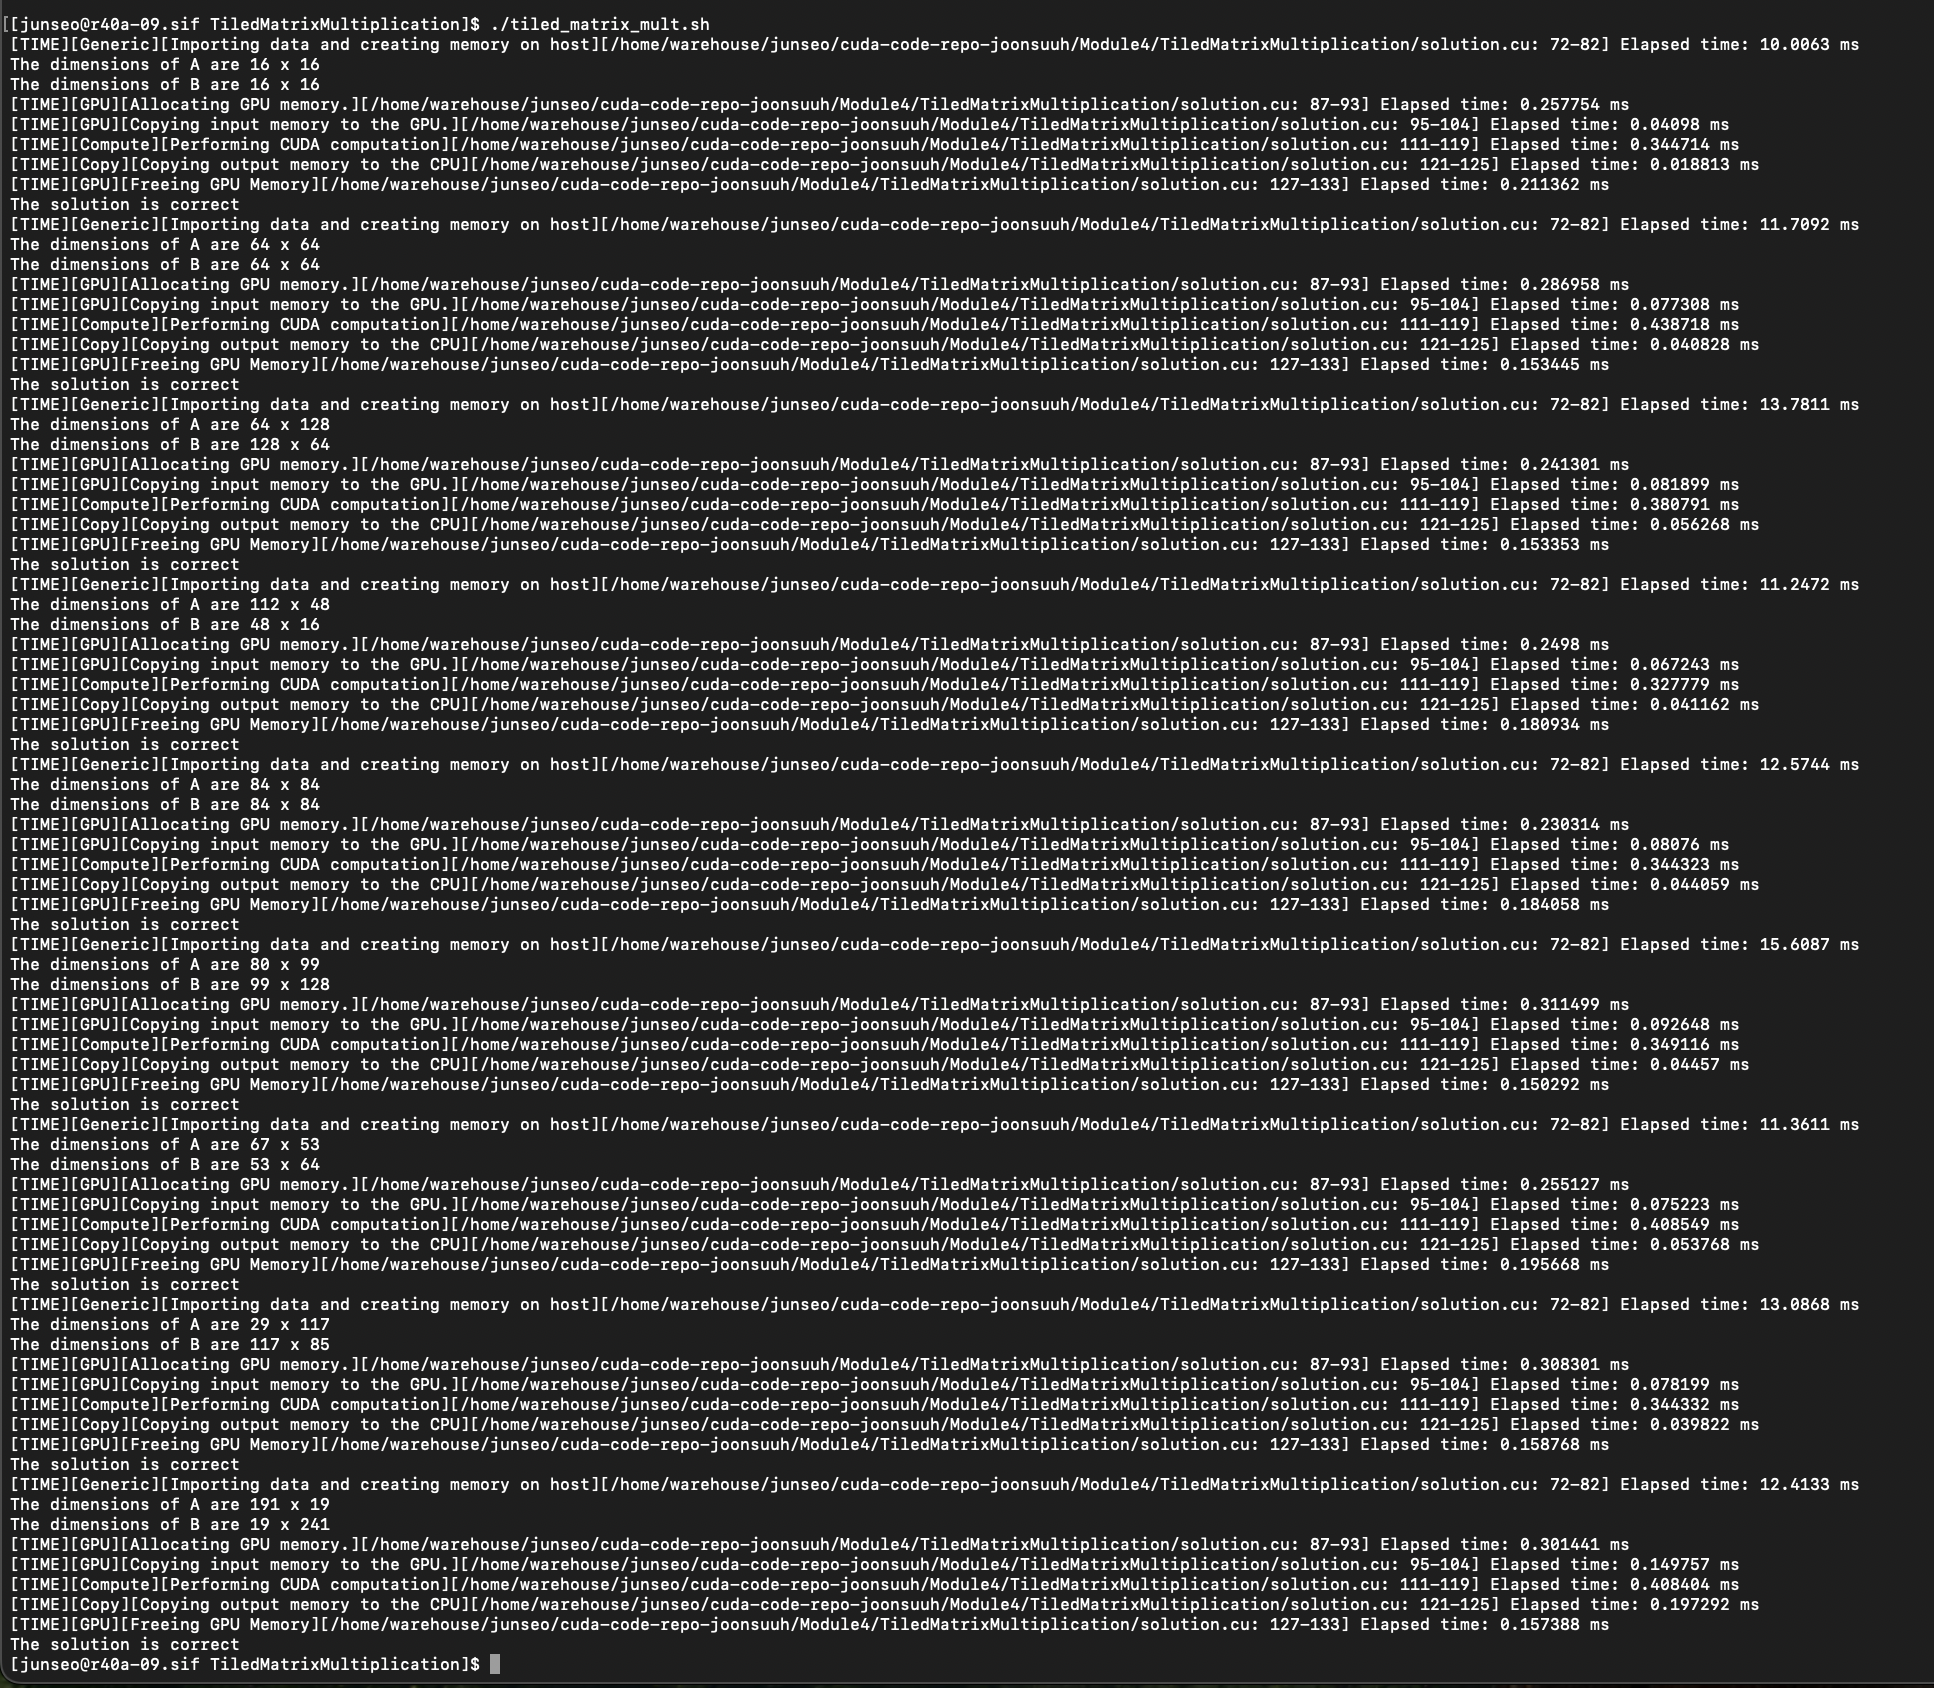
\includegraphics[width=\textwidth]{tiledMatrixMult.png}
    \caption{\texttt{TiledMatrixMultiplication\_Solution} output}
\end{figure}
\end{document}